160. \begin{figure}[ht!]
\center{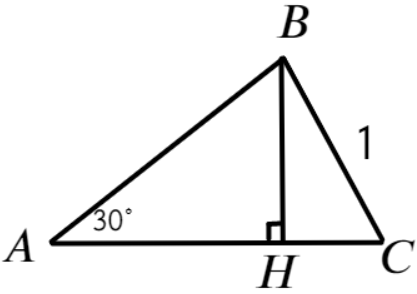
\includegraphics[scale=0.35]{g8-160.png}}
\end{figure}\\
Опустим высоту $BH,$ тогда в треугольнике $ABH$ катет $BH$ находится напротив угла в $30^\circ,$ а значит $BH=\cfrac{1}{2}AB.$ В треугольнике $BHC$ отрезок $BC$ является гипотенузой, значит $BH\leqslant BC,\ \cfrac{1}{2}AB \leqslant 1,\ AB \leqslant2.$ Равенство достигается, если $BH$ совпадает с $BC,$ то есть угол $C$ является прямым.\\
